\documentclass[10pt,letterpaper]{article}
\usepackage[top=0.85in,left=2.75in,footskip=0.75in,marginparwidth=2in]{geometry}

% use Unicode characters - try changing the option if you run into troubles with special characters (e.g. umlauts)
\usepackage[utf8]{inputenc}

\usepackage{listings}
\usepackage{float}

% clean citations
\usepackage{cite}

% hyperref makes references clicky. use \url{www.example.com} or \href{www.example.com}{description} to add a clicky url
\usepackage{nameref,hyperref}

% line numbers
\usepackage[right]{lineno}

% improves typesetting in LaTeX
\usepackage{microtype}
\DisableLigatures[f]{encoding = *, family = * }

% text layout - change as needed
%\raggedright
\setlength{\parindent}{0.5cm}
\textwidth 5.25in 
\textheight 8.75in

% Remove % for double line spacing
%\usepackage{setspace} 
%\doublespacing

% use adjustwidth environment to exceed text width (see examples in text)
\usepackage{changepage}

% adjust caption style
\usepackage[aboveskip=1pt,labelfont=bf,labelsep=period,singlelinecheck=off]{caption}

% remove brackets from references
\makeatletter
\renewcommand{\@biblabel}[1]{\quad#1.}
\makeatother

% headrule, footrule and page numbers
\usepackage{lastpage,fancyhdr,graphicx}
\usepackage{epstopdf}
\pagestyle{myheadings}
\pagestyle{fancy}
\fancyhf{}
\rfoot{\thepage/\pageref{LastPage}}
\renewcommand{\footrule}{\hrule height 2pt \vspace{2mm}}
\fancyheadoffset[L]{2.25in}
\fancyfootoffset[L]{2.25in}

% use \textcolor{color}{text} for colored text (e.g. highlight to-do areas)
\usepackage{color}

% define custom colors (this one is for figure captions)
\definecolor{Gray}{gray}{.25}

% this is required to include graphics
\usepackage{graphicx}

% use if you want to put caption to the side of the figure - see example in text
\usepackage{sidecap}

% use for have text wrap around figures
\usepackage{wrapfig}
\usepackage[pscoord]{eso-pic}
\usepackage[fulladjust]{marginnote}
\reversemarginpar

%%\usepackage{biblatex}
%%\addbibresource{preprint.bib}

% document begins here
\begin{document}
\vspace*{0.35in}

% title goes here:
\begin{flushleft}
{\Large
\textbf\newline{xml2jupyter: Mapping parameters between XML and Jupyter widgets}
}
\newline
% authors go here:
\\
Randy Heiland\textsuperscript{1},
Daniel Mishler\textsuperscript{1},
Tyler Zhang\textsuperscript{1},
Eric Bower\textsuperscript{1},
Paul Macklin\textsuperscript{1,*}
\\
\bigskip
\bf{1} Intelligent Systems Engineering, Indiana University
\bigskip
\\
*Paul.Macklin@MathCancer.org 

\end{flushleft}

\section*{Abstract}
Jupyter Notebooks \cite{Kluyver:2016aa,Nature_2018_Jupyter} provide
executable documents (in a variety of programming languages) that can be
run in a web browser. When a notebook contains graphical widgets, it
becomes an easy-to-use graphical user interface (GUI). Many scientific
simulation packages use text-based configuration files to provide
parameter values and run at the command line without a graphical
interface. Manually editing these files to explore how different values
affect a simulation can be burdensome for technical users, and
impossible to use for those with other scientific backgrounds.
xml2jupyter is a Python package that addresses these scientific
bottlenecks. It provides a mapping between configuration files,
formatted in the Extensible Markup Language (XML), and Jupyter widgets.
Widgets are automatically generated from the XML file and these can,
optionally, be incorporated into a larger GUI for a simulation package,
and optionally hosted on cloud resources. Users modify parameter values
via the widgets,
and the values are written to the XML configuration file which is input
to the simulation's command-line interface. xml2jupyter has been tested
using PhysiCell \cite{PhysiCell:2018}, an open source, agent-based
simulator for biology, and it is being used by students for classroom
and research projects. In addition, we use xml2jupyter to help create
Jupyter GUIs for PhysiCell-related applications running on nanoHUB \cite{nanoHUB_2013}.

\section*{Introduction}
A PhysiCell configuration file defines model-specific
\texttt{\textless{}user\char`_parameters\textgreater{}} in XML. Each
parameter element consists of its name with attributes, defining its
data \emph{type}, \emph{units} (optional), \emph{description}
(optional), whether the widget should be \emph{hidden} (optional), and
the parameter's default value. The attributes will determine the
appearance and behavior of the Jupyter widget. For numeric widgets (the
most common type for PhysiCell), xml2jupyter will calculate a delta step
size as a function of the default value and this step size will be used
by the widget's graphical increment/decrement feature.

To illustrate, we show the following simple XML example, containing each
of the four (currently) supported data types and the various attributes:

\begin{verbatim}
<PhysiCell_settings>
  <user_parameters>
    <radius type="double" units="micron"
        description="initial tumor radius">250.0
    </radius>
    <threads type="int">8</threads>
    <color type="string" hidden="true">red</color>
    <fix_persistence type="bool">True</fix_persistence>
  </user_parameters>
</PhysiCell_settings>
\end{verbatim}

When we map this into Jupyter widgets, we obtain the rendered results in
Figure 1. Notice the \texttt{color} parameter is not displayed since we
specified it should be hidden in the XML. The name of the other
parameters, their values, and attributes, if present, are displayed in
rows (as disabled Jupyter button widgets). Using alternating row colors
(``zebra stripes'') helps visually match associated fields and avoid
changing the wrong parameter value. For numeric widgets (type ``int'' or
``double''), we compute a delta step value based on the magnitude (log)
of the initial value. For example, the \texttt{radius} widget will have
a step value of 10, whereas \texttt{threads} will have a step value of
1.

\begin{figure}[H]
\centering
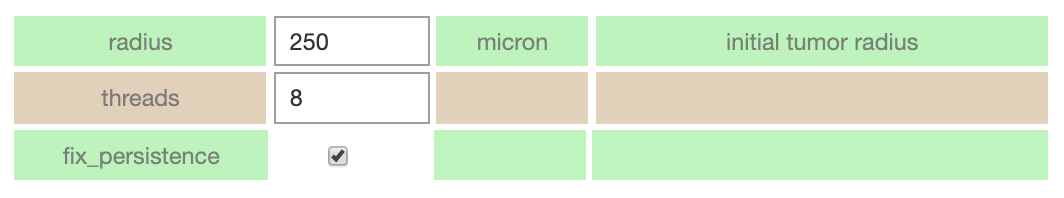
\includegraphics[width=1.0\textwidth]{images/simple_widgets.png}
\caption{Simple example of XML parameters as Jupyter widgets.}
\end{figure}

For a more realistic example, consider the
\texttt{config\char`_biorobots.xml} configuration file (found in the
\texttt{config\char`_samples} directory). The XML elements in the
\texttt{\textless{}user\char`_parameters\textgreater{}} block include the
(optional) \emph{description} attribute which briefly describes the
parameter and is displayed in another widget. To demonstrate xml2jupyter
on this XML file, one would: 1) clone or download the repository, 2)
copy the XML configuration file to the root directory, and 3) run the
\texttt{xml2jupyter.py} script, providing the XML file as an argument.

\begin{verbatim}
$ cp config_samples/config_biorobots.xml .
$ python xml2jupyter.py config_biorobots.xml 
\end{verbatim}

\begin{sloppypar}
The \texttt{xml2jupyter.py} script parses the XML and generates a Python
module, 
\texttt{user\char`_params.py}, 
containing the Jupyter widgets,
together with methods to populate their values from the XML and write
their values back to the XML. To ``validate'' the widgets were generated
correctly, one could, minimally, open \texttt{user\char`_params.py} in an
editor and inspect it.
\end{sloppypar}

But to actually see the widgets rendered in a notebook, we provide a
simple test:

\begin{verbatim}
$ python xml2jupyter.py config_biorobots.xml test_user_params.py
$ jupyter notebook test_gui.ipynb
\end{verbatim}

This should display a minimal notebook in your browser and, after
selecting \texttt{Run\ all} in the \texttt{Cell} menu, you should see
the notebook shown in Figure 2.

\begin{figure}
\centering
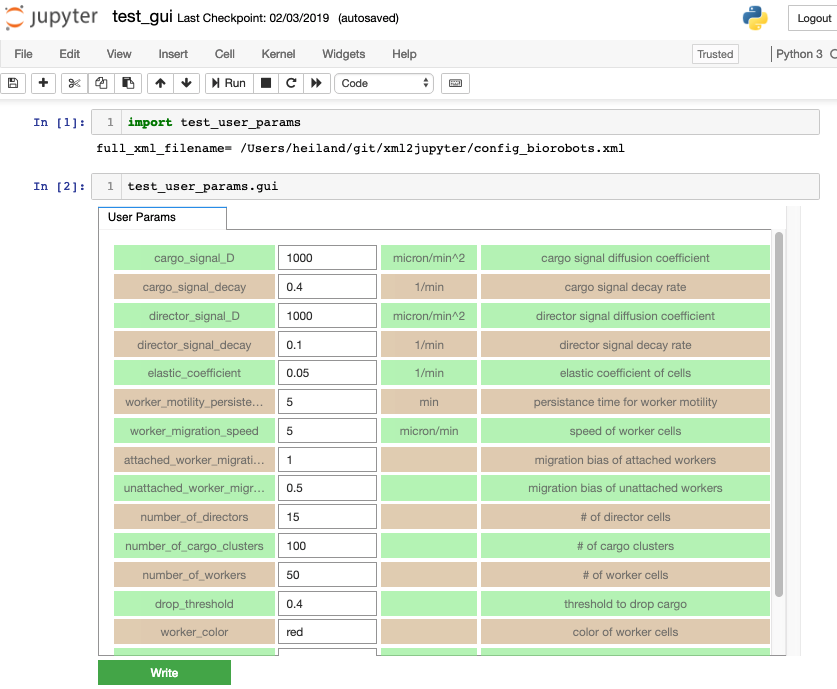
\includegraphics[width=1.0\textwidth]{images/test_biorobots_params.png}
\caption{The biorobots parameters rendered as Jupyter widgets.}
\end{figure}

\section*{PhysiCell Jupyter GUI}

Our ultimate goal is to generate a fully functional GUI for PhysiCell
users. xml2jupyter provides one important piece of this - dynamically
generating widgets for custom user parameters for a model. By adding
additional Python modules to provide additional components (tabs) of the
GUI that are common to all PhysiCell models, a user can configure, run,
and visualize output from a simulation. Two tabs that provide
visualization of output files are shown below with results from the
\emph{biorobots} simulation. Note that some of the required modules are
not available in the Python standard library, e.g., Matplotlib \cite{Hunter:2007}
and SciPy \cite{Jones:2001}. 2001). We provide instructions for
installing these additional dependencies in the repository README.

\begin{figure}
\centering
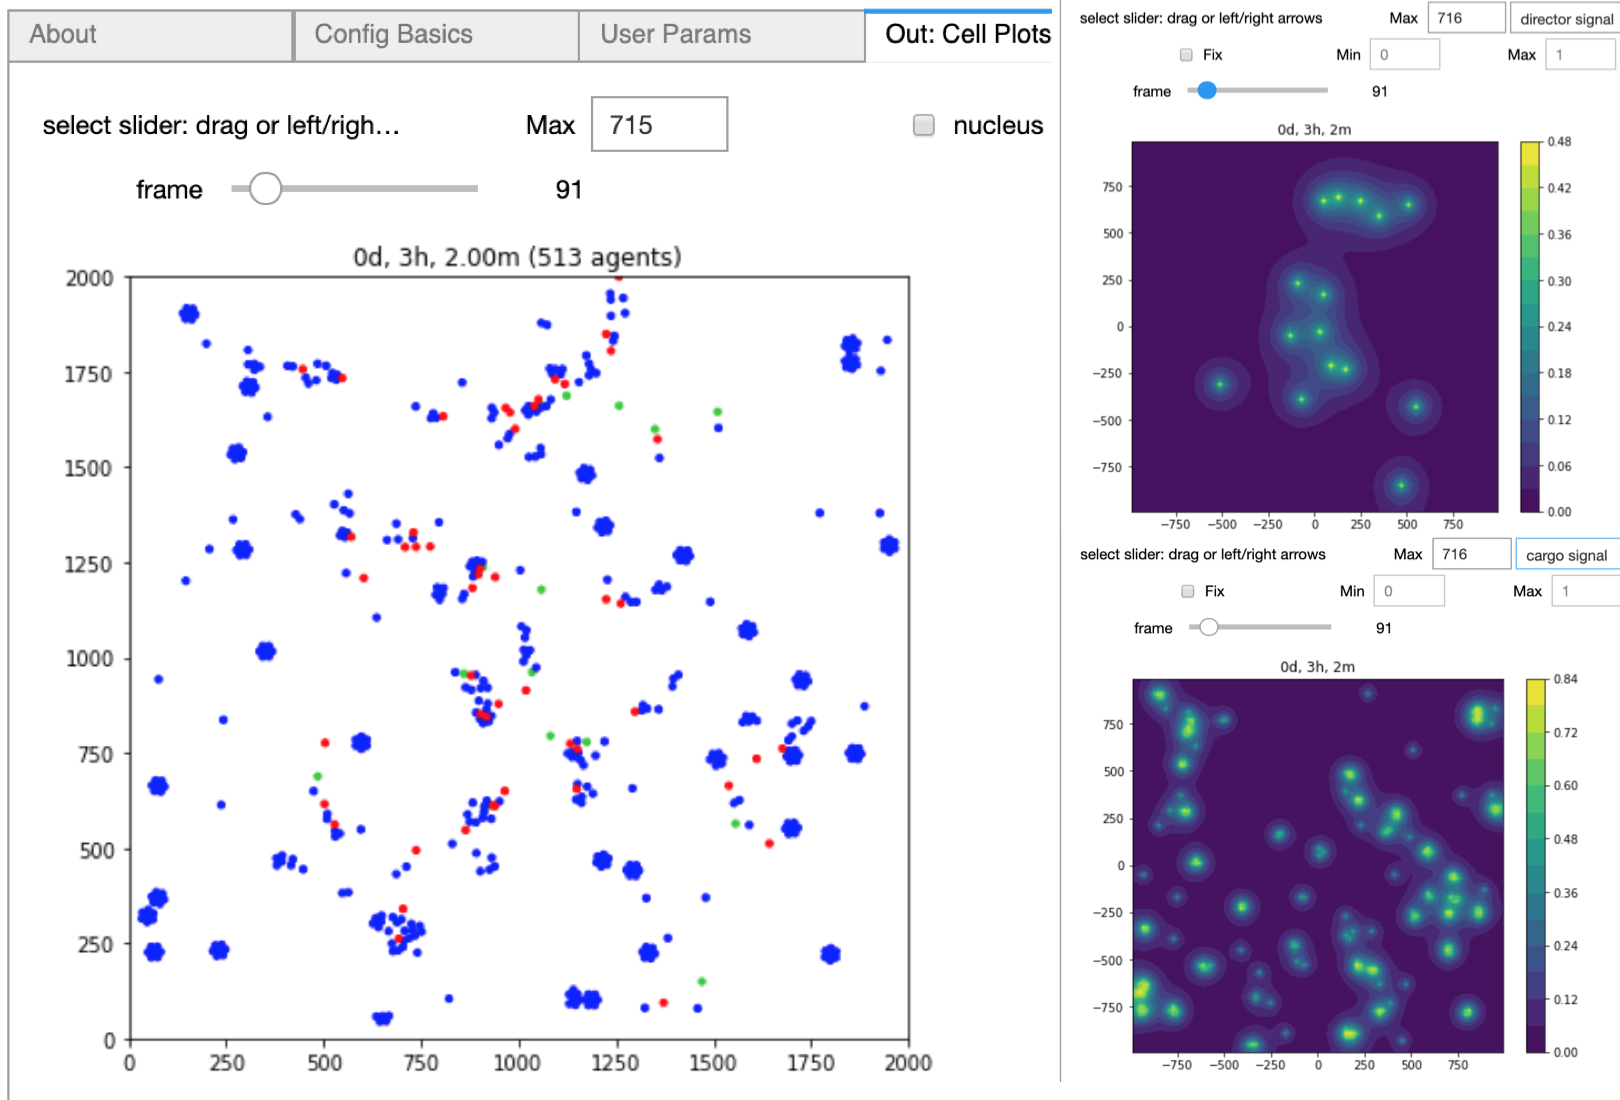
\includegraphics[width=1.0\textwidth]{images/biorobots_About_montage.png}
\caption{Plotting the biorobots (cells; left) and signals (substrates;
right).}
\end{figure}

\section*{Extensions and Discussion}

We hope others will be inspired to extend the core idea of this project
to other text-based configuration files. XML is only one of several
data-interchange formats, and while we
created this tool for XML-based configurations based on needs to create
GUIs for PhysiCell projects, the approach should be more broadly
applicable to these other formats. And while the additional Python
modules that provide visualization are also tailored to PhysiCell
output, they can serve as templates for other scientific applications
whose input and output file formats provide similar functionality.

xml2jupyter has helped us port PhysiCell-related Jupyter tools to
nanoHUB, a scientific cloud for nanoscience education and research that
includes running interactive simulations in a browser. For example,
Figure 4 shows the xml2jupyter-generated \emph{User Params} tab in our
our
\href{https://nanohub.org/tools/pc4cancerbots}{\texttt{pc4cancerbots}}
tool running on nanoHUB. Figure 5 shows the cells (upper-left) and three
different substrate plots for this same tool. This particular model and
simulation is described in this
\href{https://www.youtube.com/watch?v=wuDZ40jW__M}{video}.

Other PhysiCell-related nanoHUB tools that have been created using
xml2jupyter include
\href{https://nanohub.org/tools/pc4heterogen}{\texttt{pc4heterogen}},
\href{https://nanohub.org/tools/pcisa}{\texttt{pcISA}}, and
\href{https://nanohub.org/tools/pc4cancerimmune}{\texttt{pc4cancerimmune}}.
Readers can create a free account on nanoHUB and run these simulations
for themselves. We encourage students to use xml2jupyter to create their
own nanoHUB tools of PhysiCell models that 1) can be run and evaluated
by the instructor, 2) can be shared with others, and 3) become part of a
student's living portfolio. (Another repository,
\url{https://github.com/rheiland/tool4nanobio}, provides instructions
and scripts to help generate a full GUI from an existing PhysiCell
model.)

\begin{figure}
\centering
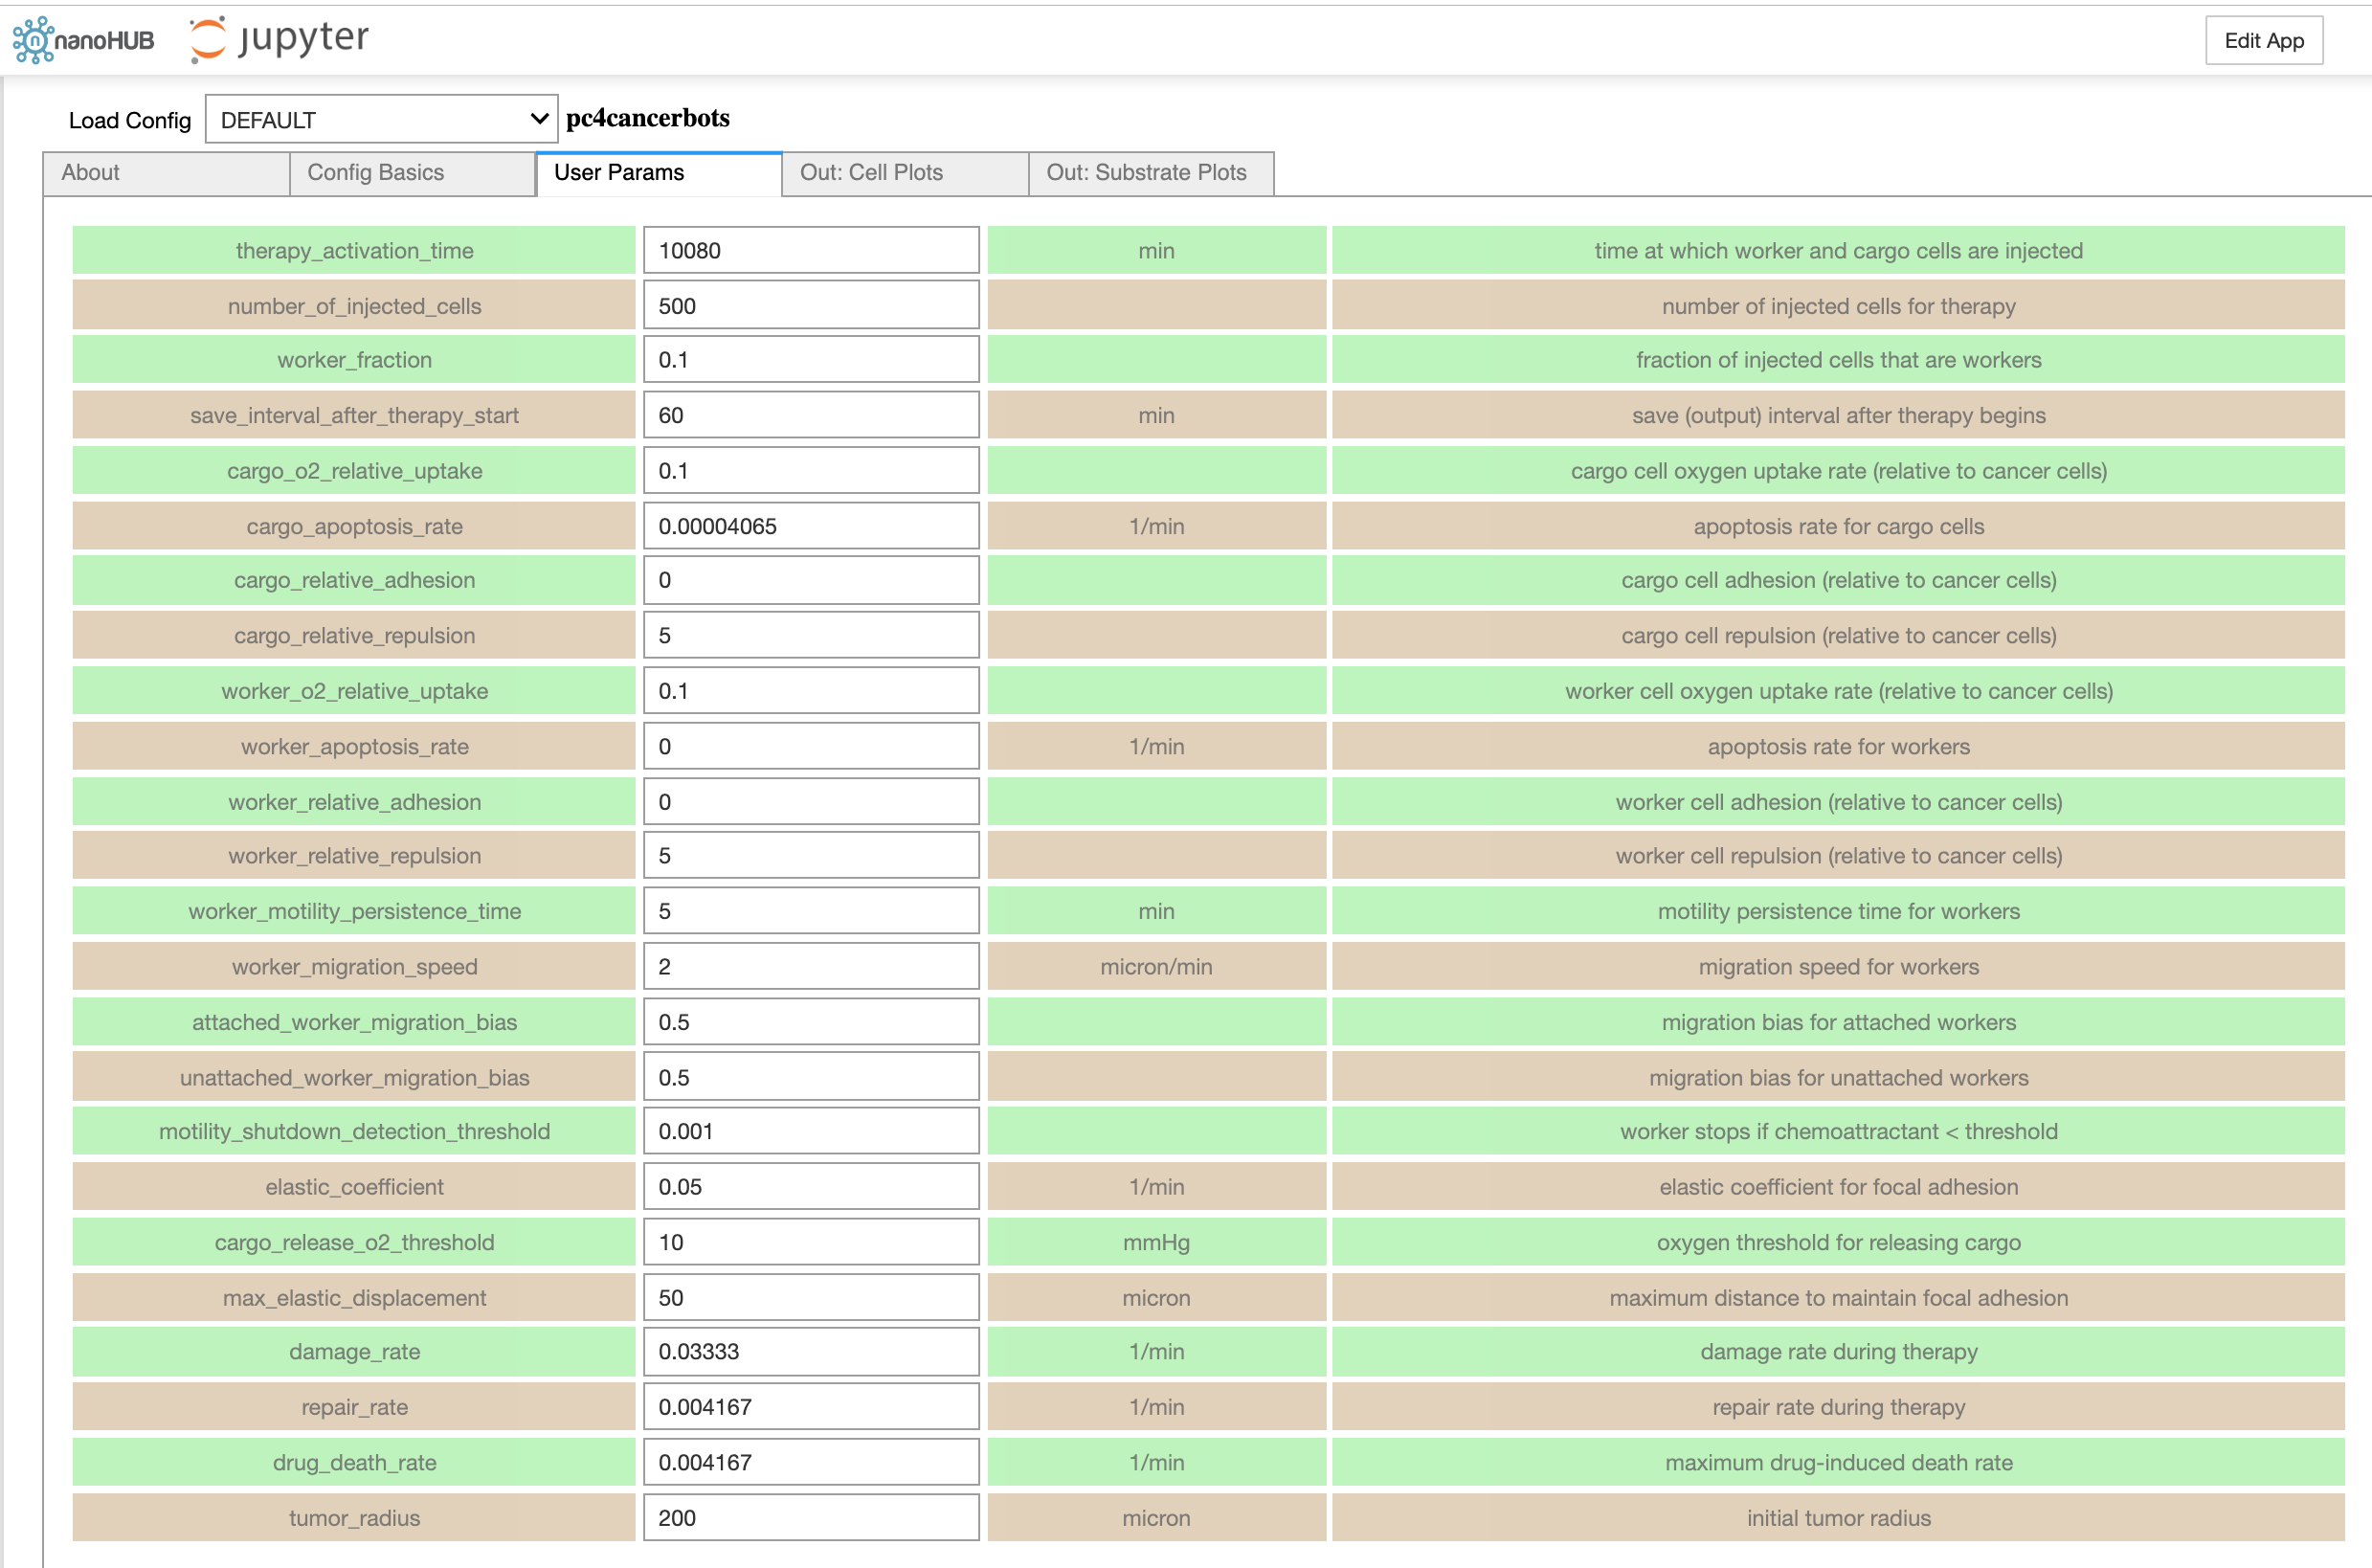
\includegraphics[width=1.0\textwidth]{images/nanohub_cancerbots_params.png}
\caption{The cancer biorobots parameters in a nanoHUB Jupyter
application.}
\end{figure}

\begin{figure}
\centering
%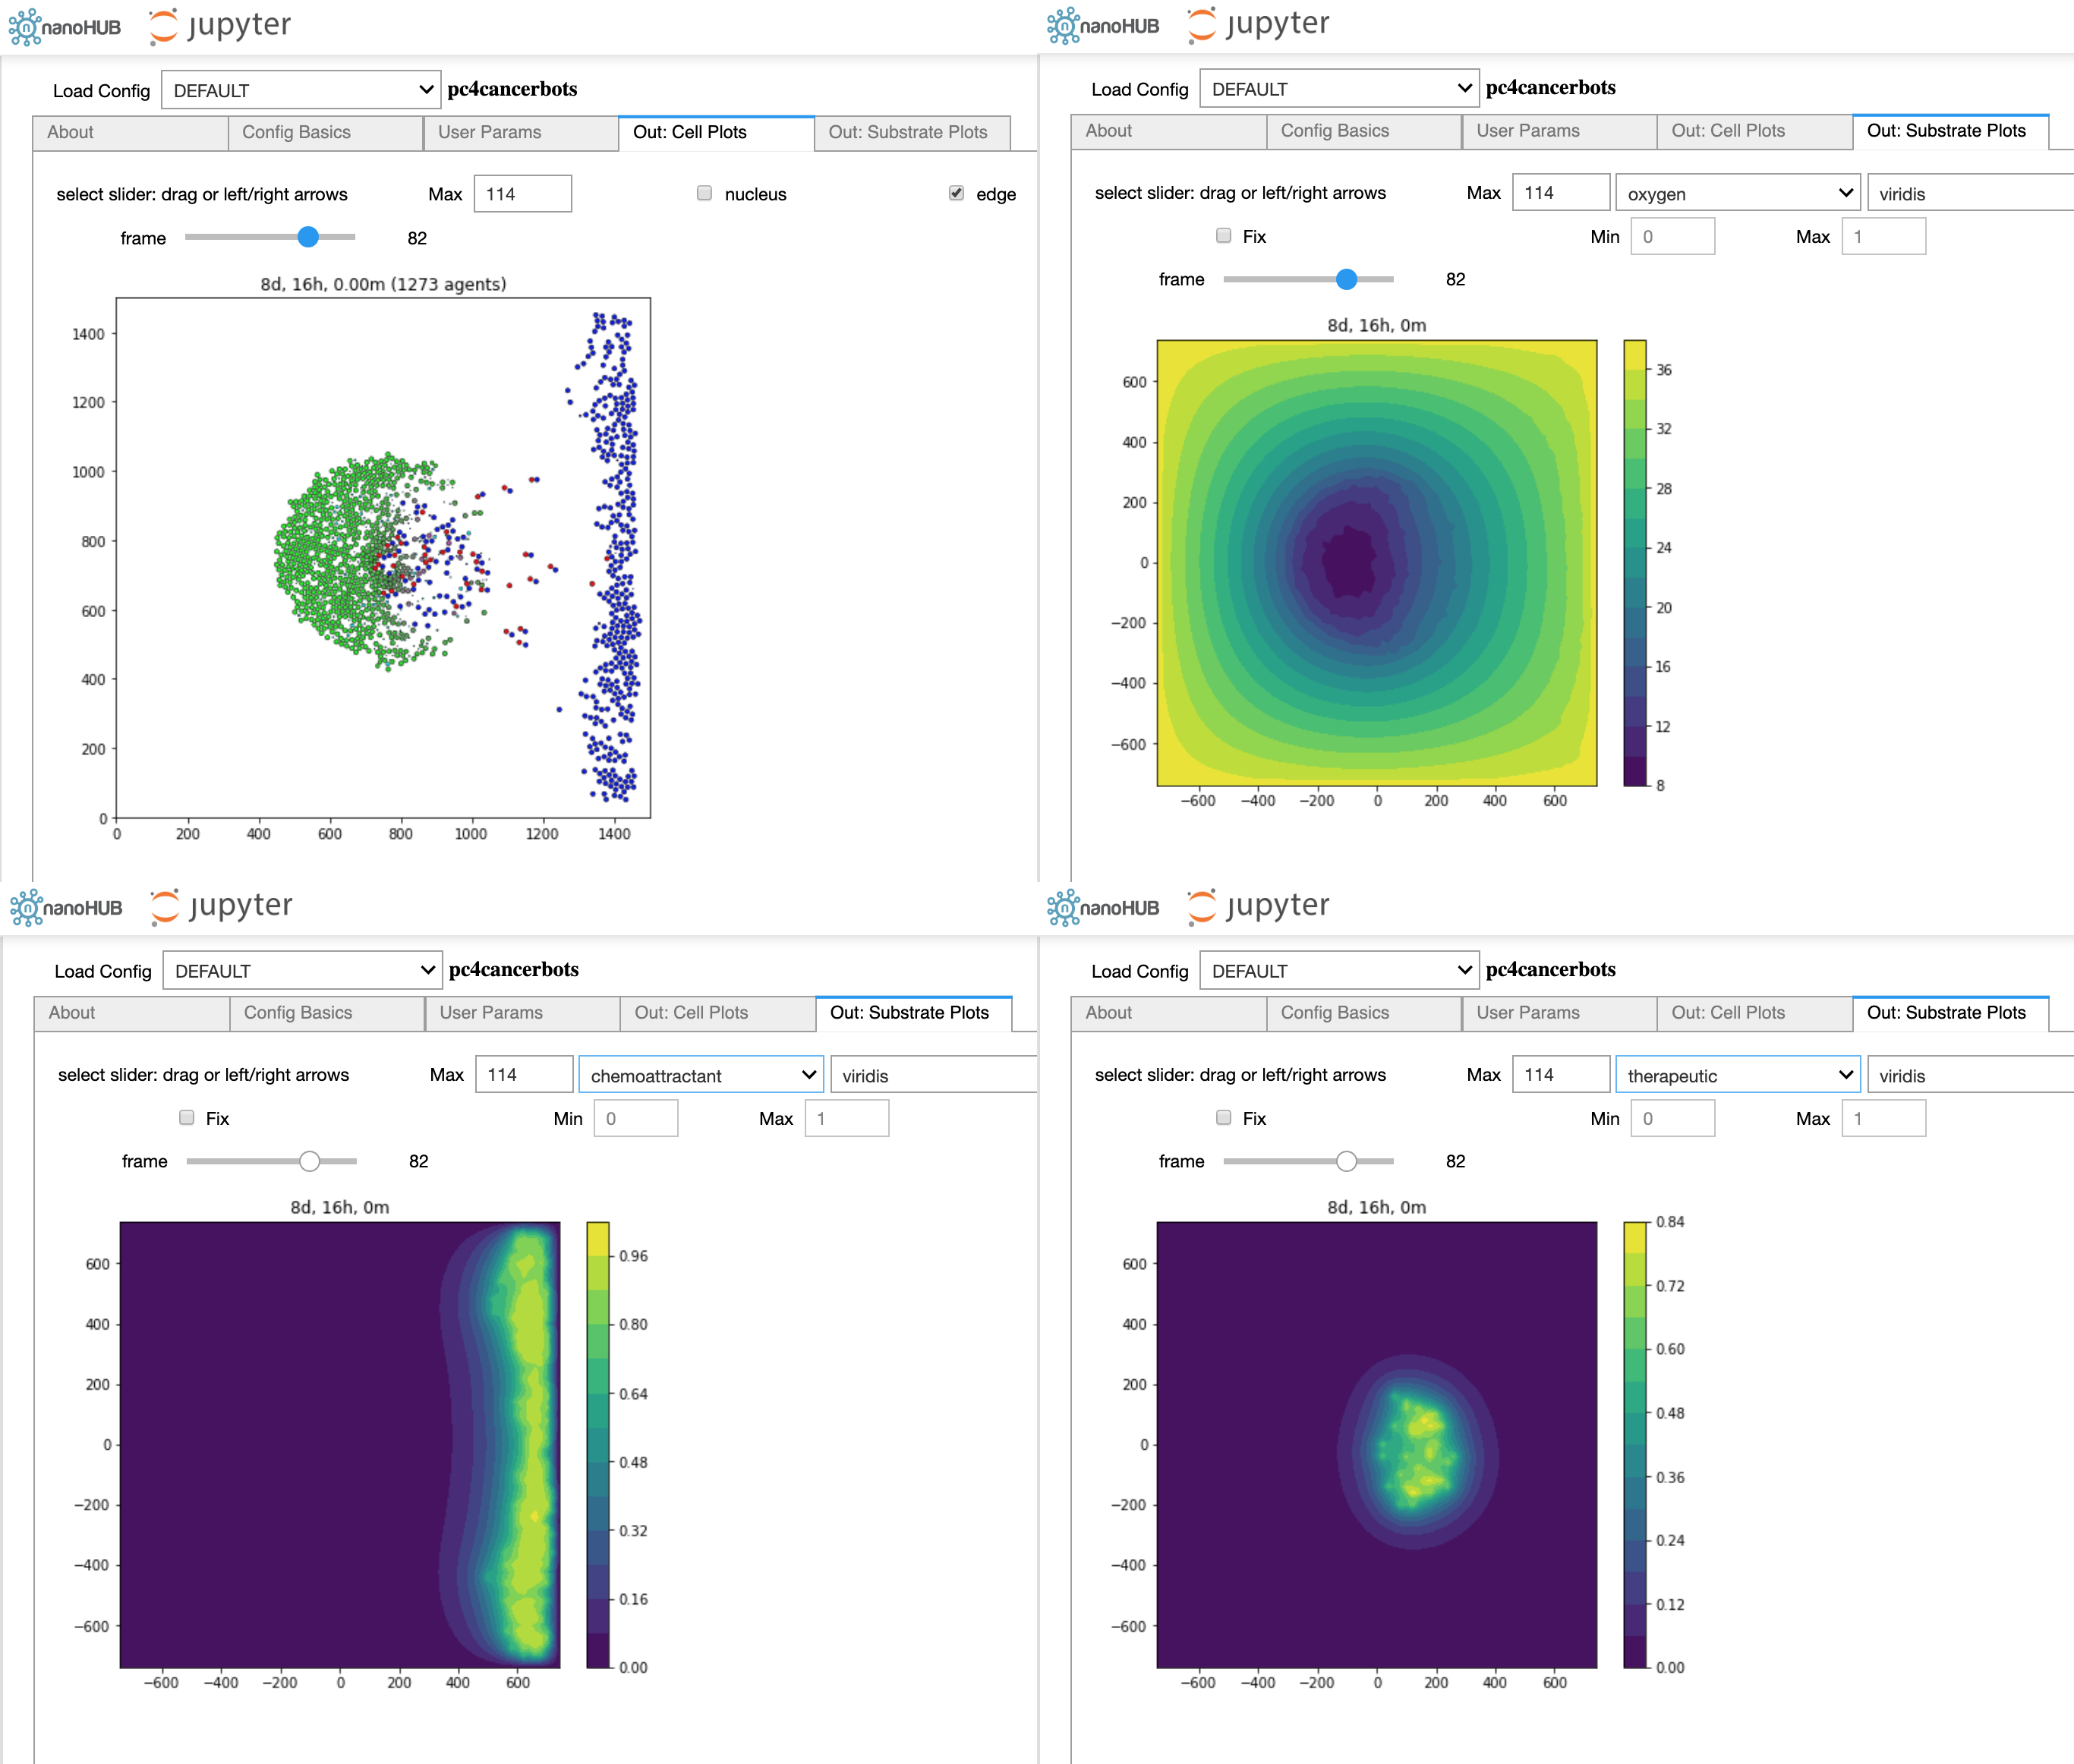
\includegraphics[scale=0.2]{images/nanohub_cancerbots_2x2.png}
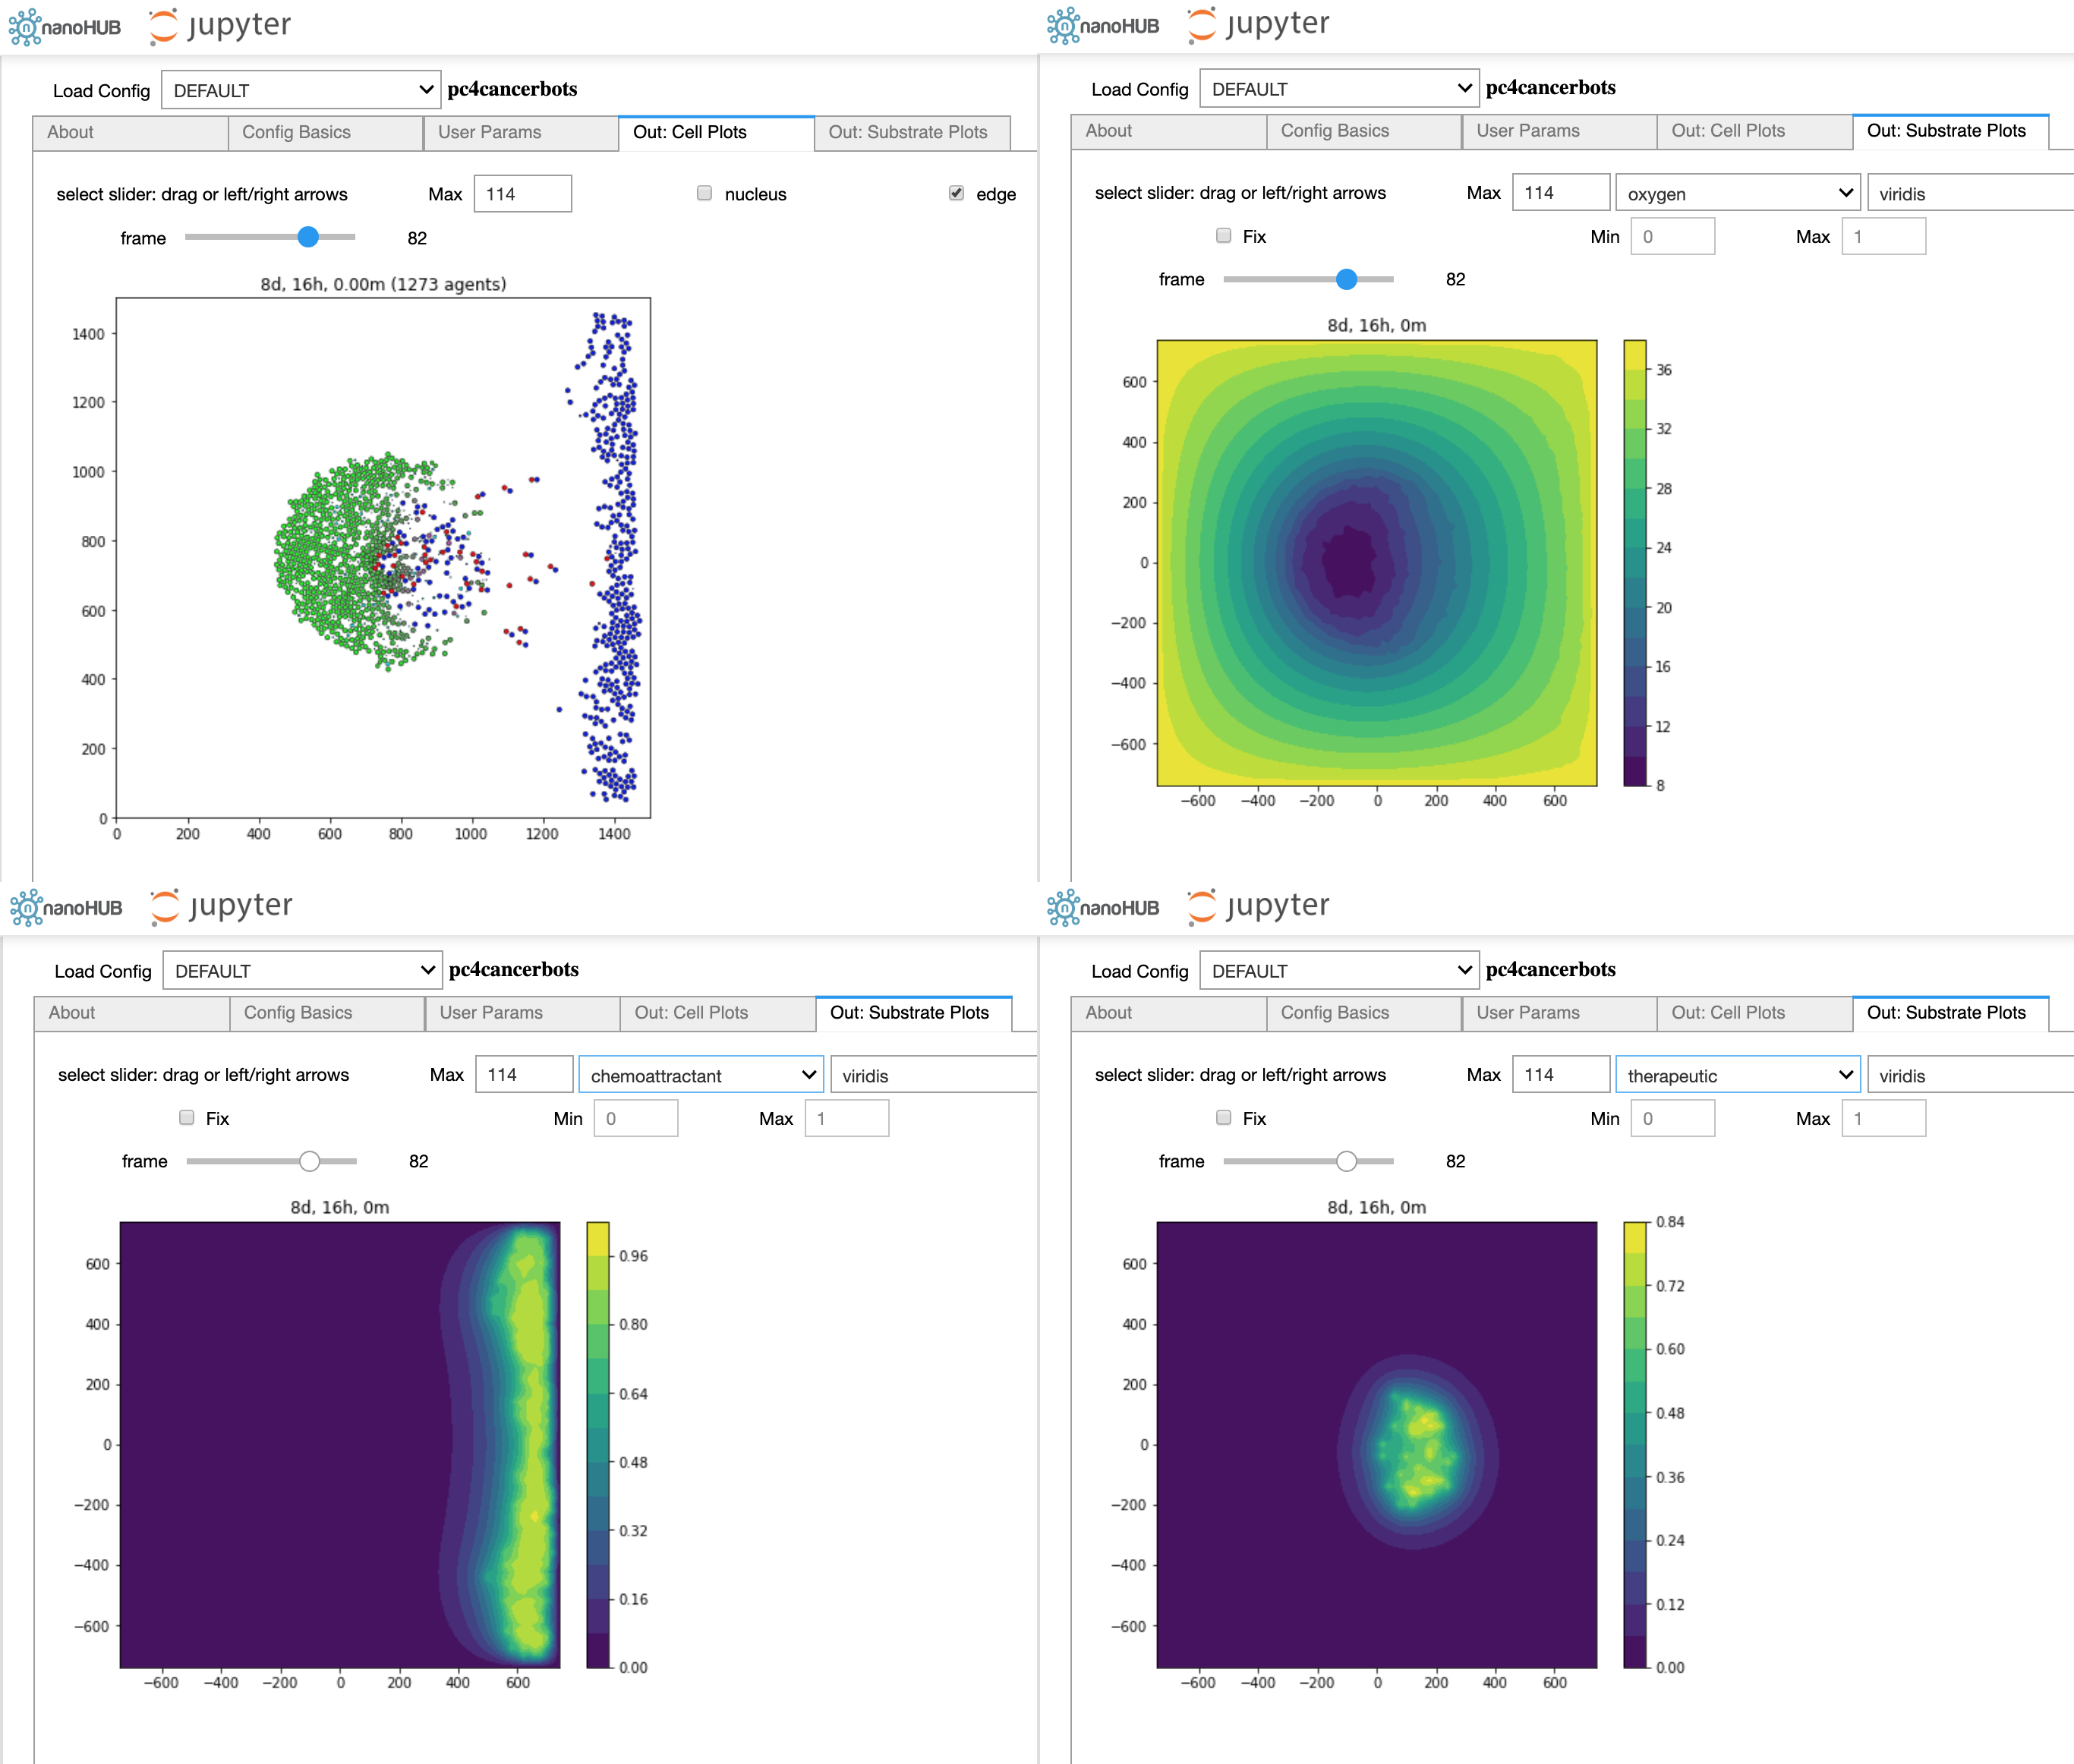
\includegraphics[width=1.0\textwidth]{images/nanohub_cancerbots_2x2.png}
\caption{The cancer biorobots Jupyter notebook on nanoHUB.}
\end{figure}

We welcome suggestions and contributions to xml2jupyter. For example,
currently, we arrange the generated parameter widgets vertically, one
row per parameter. This is an appropriate layout for an educational
setting. But if a GUI will be used by researchers who are already
familiar with the parameters, it may be preferable to generate a more
compact layout of widgets, e.g., in a matrix with only the parameter
names and values. Moreover, it may be useful to provide additional
control over styling and placement by a separate style.xml or similar
file, or by an external cascading style sheet. We will explore these
options in the future, with the aim of separating as much GUI
specification and styling from the original scientific application as
possible. Such a decoupling would make it easier for scientific
developers to continue refining their scientific codes without worrying
about impact on the GUI, and without undue encumbrance by non-scientific
annotations.

Also, we currently provide just 2-D visualizations of (spatial) data. In
the near future, we will provide visualizations of 3-D models and
welcome suggestions from the community.

\section*{Acknowledgements}

We thank the National Science Foundation (1720625) and the National
Cancer Institute (U01-CA232137-01) for generous support. Undergraduate
and graduate students in the Intelligent Systems Engineering deparment
at Indiana University provided internal testing, and students and
researchers within the NSF nanoMFG (1720701) group generously provided
external testing. All of their feedback resulted in considerable
improvements to this project. Finally, we thank our collaborators at
Purdue University, especially Martin Hunt and Steve Clark, who provided
technical support with nanoHUB and Jupyter.

%%This defines the bibliographies style. Search online for a list of available styles.
\bibliographystyle{abbrv}
\bibliography{preprint}   % .bib


\end{document}